\section*{فرصتی برای مدل‌های دیگر نورونی}
در بخش قبل به بررسی ویژگی‌های مدل انباشت‌-شلیک پراختیم. اگر چه این مدل بسیار ساده توانست رفتارهای آشنایی را برای ما بازتولید کند اما شامل محدودیت‌هایی است. این محدودیت‌ها باعث می‌شود تا ما به سراغ مدل‌های نورونی دیگری مانند نورون‌های چرخنده برویم.\\
این مدل نسبت به مدل قبلی شامل ویژگی‌های مثبتی است. یکی از ویژگی‌های خوب آن این است که پس از بازنشانی فاز نورون تیزه زده، فاز آن به زاویه‌ای برده می‌شود که دارای خواص مثلثاتی مشابهی است. به این معنا که دیگر شاهد گسستگی در اندازه‌ی جملاتی که تحول نورون را توصیف می‌کنند؛ نیستیم.\\

\فصل{شبکه‌ی نورون‌های چرخنده}
\label{chap:rotational}
در این مدل به جای آن که برای شبکه خود از مدل انباشت-شلیک استفاده کنیم از مدل چرخنده استفاده می‌کنیم. در این مدل نورون‌های ما مانند دونده‌هایی به دور دایرهٔ مثلثاتی می‌دوند. ما نقطه‌ی فاز $\pi$ را به عنوان علامت برای این دونده‌ها قرار دادیم. هر زمان که دونده‌ای از علامت خود گذشت یک تیزه برای او درنظرمی‌گیریم و بلافاصله او را به فاز $-\pi$ باز می‌گردانیم.\\

برای توصیف فاز هر نورون از معادلات زیر استفاده می‌کنیم:
\begin{tcolorbox}
	\begin{equation}
		\begin{cases}
			\dot{\theta_i}=I_i - \cos{\theta_i} - g E, \hspace{2ex} \theta_i \leq \pi \\
			\dot{E} = M - \alpha E\\
			\dot{M} = -  \alpha M + \frac{ \alpha^{2} }{N} \sum_{n|t_{n}<t} \delta(t - t_n - t_d)
		\end{cases}
	\end{equation}
	\begin{enumerate}[-]
		\item $\theta_i$:
		مشخص کننده‌ی فاز هر نورون. این فاز میان دو لبه در حال حیات است. کوچکترین کران بالای آن همان حالت آستانه در $\pi$ است و بزرگترین کران پایین آن نگه‌دارنده‌ای است که از ریزش نورون‌ها جلوگیری می‌کند.
		\item $E$:
		میدانی است که شدت فعالیت شبکه را نشان می‌دهد.
		\item $M$:
		یک پارامتر فرعی که در حل معادله دیفرانسیل مرتبه دوم به دو معادلهٔ تحول مرتبه اول ما را یاری کرده است.
	\end{enumerate}
\end{tcolorbox}

\قسمت{آهنگ تیزه زدن}
برای نورونی تنها که پویایی از جنس چرخنده دارد؛ دوره‌ی تناوب و بسامد تیزه زدن آن برحسب مجموع جریان ورودی‌ رفتاری مطابق زیر دارد (پیوست
\ref{appendix:activity_calculation}):

\begin{align}
	T &= \frac{2\pi}{\sqrt{I^2 - 1}},\\
	f &= \frac{1}{T} = \frac{\sqrt{I^2 - 1}}{2\pi}.
\end{align}
این به این معناست که مدل چرخنده و انباشت‌وشلیک اگر چه هر دو با افزایش جریان، بسامد تیزه زدنشان افزایش می‌یابد اما رفتار تغییر آن به دو گونه‌ی متفاوت صورت می‌پذیرد. این نکته‌ی مهمی است که در هنگام مقایسه‌ی دو مدل باید به خاطر داشته باشیم.

\قسمت{نشانگر توسعه یافته‌ی تشخیص همگامی}
گفتنی است که برای تشخیص هم‌گامی می‌توان پارامترهای دیگری نیز استفاده کرد. به عنوان مثال در مرجع
\cite{safaeesirat2020critical}
 پارامتر دیگری توسط نویسندگان ابداع و معرفی شده‌است،

\begin{equation}
	s =  \braket{ \big[ \frac{1}{N_a}\sum_{i_a} sin(\theta_{i_a}) \big]^{2}}_t
	\label{eq:saman_amin_param}
\end{equation}
میانگین‌گیری بالا روی ۱۰۰۰ گام آخر زمانی انجام می‌شود. این فاصله زمانی باید حتما بزرگ‌تر از گام‌های زمانی تحول ریزمقیاس آن باشد. همچنین برای این متوسط‌گیری نورون‌هایی را مدنظر می‌گیریم که در منطقه ی فعال قرار گرفته‌اند. منطقه‌ی فعال، سمت چپ دایره مثلثاتی است. تعداد این نورون‌ها را با $N_a$ نمایش می‌دهیم.\\
برای پی بردن به فایده‌ی این مشخصه آن را در مرحله‌ی آزمایش ذهنی قرار می‌دهیم. دو حالت از سامانه در حالت هم‌گام و نا‌هم‌گام را در نظر می‌گیریم و استدلال می‌کنیم که این مشخصه تفاوت آن‌ها را به روشنی آشکار می‌کند.\\

\begin{enumerate}[(a)]
	\item 
	حالتی که همه‌ی نورون‌ها روی دایره‌ی مثلثات به صورت یکنواخت توزیع شده‌اند: به وضوح در چنین حالتی به علت فرد بودن تابع سینوس نتیجه‌ی رابطه‌ی یاد شده صفر خواهد بود. پس این رابطه عدد صفر را برای حالت مطلق نا‌هم‌گامی در نظر می‌گیرد.
	\item 
	حالتی از نورون‌ها که همه در یک فاز قرار دارند و با هم روی دایره می‌دوند: در چنین حالتی میانگین زمانی مشخصه‌ی s برابر عدد ۱/۲ است.
	\item 
	گفتنی است که بقیه حالات توزیع نورون‌ها میان این دو حالت لبه‌ای قابل تصور هستند و خروجی این مشخصه عددی بین صفر و ۱/۲ خواهد بود.
\end{enumerate}

\قسمت{شبیه‌سازی}
ثوابت مسئله را به گونه‌ی زیر انتخاب می‌کنیم.
\begin{tcolorbox}[colback=green!5!white,colframe=green!75!black]
	\begin{enumerate}[*]
		\item
		$\alpha = 20$
		\item
		جریان‌های تصادفی خارجی نورون‌ها از اعضای بازه‌ی $(9.5,13.5)$ انتخاب می‌شوند. بیشینه‌ی (کمبنه) این بازه به گونه‌ای انتخاب شده‌است که فعالیت نورونی متصل به آن‌ کاملا مشابه نورون انباشت‌وشلیکی باشد که بیشینه‌ی (کمینه) جریان را در بخش قبل داشت. 
		\item
		$N = 10^4$
		\item
		$t_d = 0.1$ 
	\end{enumerate}
\end{tcolorbox}
حال شبکه‌ی خود را به ازای قدرت اتصال‌های مختلف اجرا می‌کنیم تا مجددا تحقیق کنیم که چگونه تغییر در قدرت اتصال $g$ می‌تواند باعث شود تا تغییر فاز از ناهم‌گامی به هم‌گامی رخ دهد. برای مشاهده‌ی دفترچه شبیه‌سازی به آدرس 
\href{https://github.com/mmehrani/master_thesis/tree/main/scripts/rotational_model}{مسئله همگامی برای مدل چرخنده}
مراجعه کنید.

\قسمت{نتایج }
مرتبه‌ی اجرای این الگورتیم خطی است و برای یک شبکه شامل ۱۰۰۰ نورون و برای $10^4$ گام شبیه‌سازی زمانی در حدود ۴ ثانیه به طول می‌انجامد. 


\زیرقسمت{در جستجوی تغییرفاز}
پس از رصد کردن تغییرات رفتار سیستم بر حسب قدرت مهار نورون‌ها، تغییر فاز مانند مدل قبلی مشاهده شد اما مکان تغییر فاز تغییر کرد و حول $g=30$ قرارگرفت. این تغییر فاز در دو شکل \ref{fig:sigma_rotational} و \ref{fig:amin_saman_rotational}  قابل مشاهده‌است.\\
شاید به نظر این مسئله کمی عجیب برسد و تا حدودی مسیر حل ما را دچار چالش کند اما نکته‌ی قابل توجه برای ما تفاوت نقاط گذر فاز نیست بلکه کیفیت تغییر فاز است. صرف وجود فازی هم‌گام پس از نا‌هم‌گام قابل تامل است که برای هر دو مدل نورونی رخداده است.\\
در مورد جابجایی نقاط گذر نیز می‌توانیم با نگاه دقیق‌تر به معادلات نورون‌های انباشت‌وشلیک و چرخنده آن را دریبایم.\\

بیایید جمع دو جمله‌ی اول را برای هر مدل از شبکه‌های شبیه‌سازی شده‌ی خود در نظر بگیریم. (الف) برای شبکه‌ی انباشت‌وشلیک در بازه‌ی 
$(0.2, 2,8)$
است و برای (ب) شبکه‌ی چرخنده در بازه‌ی
$(8.5, 13.5)$
قرار دارد.\\
 همان‌طور که مشخص است مرکز این بازه‌ها در یک مرتبه‌ی بزرگی با هم تفاوت دارند. اگر کیفیت تغییرفاز برای هر دو مدل مشابه است؛ طبیعی است که تصور کنیم جمله‌ی مهاری سوم نیز در نقطه‌ی گذر باید  یک مرتبه‌ی بزرگی بین دو مدل متفاوت باشد.\\
 از آن‌جا که میدان
 $E$
 مستقل از تعداد نورون‌هاست و فقط به چگالی حضور نورون‌ها روی محور آستانه مربوط است؛ این ضریب تاثیر است که باید نقش درخواستی را ایفا کند و یک مرتبه‌ی بزرگی بین دو نورون متفاوت باشد.
\begin{figure}
	\begin{subfigure}[b]{0.5\textwidth}
	\centering
	\includegraphics[width = \textwidth]{../scripts/all_neurons_model_in_one_place/Rotational_ensembles/N10000_T100_I9.5_13.5_v1.0/sigma_g_0_130.png}
	\caption{پهنای جریان یک سامانه چرخنده با ده هزار نورون}
	\label{fig:sigma_rotational}
	\end{subfigure}
	\hfill
	\begin{subfigure}[b]{0.5\textwidth}
		\centering
		\includegraphics[width = \textwidth]{../scripts/all_neurons_model_in_one_place/Rotational_ensembles/N10000_T100_I9.5_13.5_v1.0/amin_saman_param_g_0.1_65.png}
		\caption{پارامتر نظم تعریف شده در رابطه \ref{eq:saman_amin_param} برای مدل چرخنده }
		\label{fig:amin_saman_rotational}
	\end{subfigure}
	\hfil
	\begin{subfigure}[b]{0.5\textwidth}
		\centering
		\includegraphics[width = \textwidth]{../scripts/all_neurons_model_in_one_place/Rotational_ensembles/N10000_T100_I9.5_13.5_cluster_computed/mean_spiking_persiods_g_0.1_65.png}
		\caption{فاصله‌ی زمانی بین تیزه زدن‌ها}
		\label{fig:interspikes_rotational}
	\end{subfigure}
	\hfill
	\begin{subfigure}[b]{0.5\textwidth}
		\centering
		\includegraphics[width = \textwidth]{../scripts/all_neurons_model_in_one_place/Rotational_ensembles/N10000_T100_I9.5_13.5_cluster_computed/mean_spiking_persiods_with_trending_line_g_0.1_65.png}
		\caption{محاسبه‌ی نمای بحرانی}
		\label{fig:interspikes_rotational_trending_line}
	\end{subfigure}
	\hfill
	\begin{subfigure}[b]{0.5\textwidth}
		\centering
		\includegraphics[width = \textwidth]{../scripts/all_neurons_model_in_one_place/Rotational_ensembles/N10000_T100_I9.5_13.5_cluster_computed/sigma_phase_space_contour.png}
		\caption{صفحه‌ی فاز مربوط به سامانه‌ی نورون‌های چرخنده (به شکل \ref{fig:if_g_d_phase_if_space_points_plotted}
			در پیوست نگاه کنید).
		}
		\label{fig:rot_g_d_phase_space}
	\end{subfigure}
	\caption{خانواده‌ای از نمودارهای توصیف کننده‌ی سامانه‌ی چرخنده}
\end{figure}




\زیرقسمت{فاصله زمانی بین تیزه‌ها}
حال که دیدیم برخی نورون‌ها همواره خاموش می‌مانند و یا به عبارتی دوره‌ی تیزه زدن آن‌ها بینهایت است؛ خوب است که دوره‌ی تیزه زدن‌ نورون‌های دیگر را نیز بررسی کنیم - شکل \ref{fig:interspikes_rotational}.

این شکل نمایان‌گر آن است که سامانه‌ی ما توزیعی توانی دارد. یا به عبارت دیگر رفتاری بی‌مقیاس دارد با توانی که در شکل  
\ref{fig:interspikes_rotational_trending_line}
محاسبه شده است. این توان همواره با محاسبه شیب بهترین خط گذرنده از نمودار تمام لگاریتمی آن محاسبه می‌شود.\\

همچنین توجه کنیم که با افزایش ضریب تاثیر رفتار توانی آن‌ها تغییر نمی‌کند. تنها تفاوت در چگونگی انتخاب جایگاه‌های روی خط است. هر چه ضریب تاثیر بزرگتر می‌شود نورون‌ها فاصله‌ی زمانی تیزه‌های بزرگتری را اتخاذ می‌کنند. این امر با خاصیت مهاری بودن نورون‌های شبکه هم‌خوانی خوبی دارد. زیرا با افزایش ضریب تاثیر نورون‌ها در حال کندتر شدن هستند.
\\


\زیرقسمت{فعالیت شبکه}
همان طور که دیدیم تعدادی از نورون‌ها در شبکه به حالت خاموش درمی‌آیند. قابل حدس است که اگر جمعیتی خاموش در شبکه داشته باشیم؛ احتمالا آنهایی هستند که جریان تصادفی اولیه آن‌ها از بقیه کمتر است. زیرا آهنگ تیزه زدن رابطه‌ی مستقیمی با جریان‌های ورودی به نورون دارد.\\

به هر جهت رسم نمودار فعالیت نورون‌ها بر حسب جریان‌های تصادفی اولیه‌ی آن‌ها می‌تواند اطلاعات بسیار مفیدی را از شبکه به ما بدهد. به عنوان مثال شکل \ref{fig:spikes_num_vs_background_current} نشانگر سامانه‌ای از ده هزار نورون است که با قدرت $g=50$ روی هم تاثیر می‌گذارند. این ضریب تاثیر همان‌طور که در شکل
\ref{fig:sigma_rotational}
مشخص است؛ درون فاز هم‌گام قرار دارد. خط صاف سمت چپ نمودار به وضوح گویای کندی حرکت نورون‌های با جریان پایین است.\\

بیاید درستی مقادیری را که از شبیه‌سازی به دست آمده با تخمین سرانگشتی بررسی کنیم. جریان داخلی بین نورون‌ها وابسته به فعالیت شبکه است. پس به سراغ رابطه‌ی فعالیت می‌رویم. می‌دانیم می‌توانیم جریان داخلی را نیز به کمک آن توصیف کنیم.
\begin{figure}
	\centering
	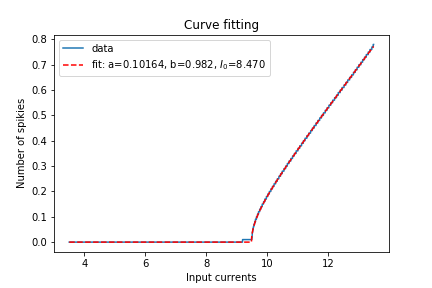
\includegraphics[width = 0.7 \textwidth]{../papers_studies/figs/Rotational/spikies_num_vs_input_fitted_curve_g50_input_3.5_13.5.png}
	\caption{تعداد تیزه برحسب جریان تصادفی برای سامانه‌ای با ده هزار نورون و ضریب تاثیر $g=50$}
	\label{fig:spikes_num_vs_background_current}
\end{figure}


تعداد تیزه‌های کل شبکه رابطه‌ی مستقیمی با جریان خارجی جاری در شبکه دارد. می‌توانیم با محاسبات تحلیلی نیز به شکل به دست آمده از شبیه‌سازی عددی نزدیک شویم:

\begin{align}
	\begin{cases}
		I_{in} &= -g \int_{a_{min}}^{a_{max}} p(a) f(a + I_{in}) da, \\
		f(a) &= \frac{\sqrt{a^2 - 1}}{2\pi}.
	\end{cases}
	\label{eq:analytical_input_current}
\end{align}

در رابطه \ref{eq:analytical_input_current} ، $f(a)$ تابع فعالیت (تعداد تیزه بر ثانیه) تک نورون بر حسب جریان کل ورودی آن است. همچنین $I_{in}$ مجموع همه‌ی جریان‌های داخلی جاری در شبکه است.\\

حل این رابطه کمی دشوار است زیرا جریان کل را بر حسب خودش محاسبه کرده است. اما از آنجایی که در انتگرال‌ده تنها یک جابجایی ثابت رخداده است؛ صورت کلی پاسخ انتگرال تغییر نمی‌کند و به صورت زیر به دست خواهد آمد.
\begin{align}
	I_{in} = \frac{-g}{2} \bigg(-a \sqrt{-1 + a^2} + log(a + \sqrt{-1 + a^2}\bigg) \Big|_{a_{min} + I_{in}}^{a_{max} + I_{in}} .
\end{align}
بی‌تردید حل معادلهٔ اخیر آشکار کننده‌ی مقدار
$I_{in}$
خواهد بود البته به شرط قابلیت حل!\\

ظاهرا گرفتن انتگرال و حل دقیق معادله کار ساده‌ای نیست. یک پیشنهاد راه حل عددی برای این مسئله این است که تابع فعالیت را با رابطه‌ی پارامتری زیر هم‌خوانی بدهیم و مقدار 
$I_0$
را پیدا کنیم،

\begin{align}
	f(I) = a \frac{\sqrt{[b(I - I_0 )]^2 - 1}}{2\pi} .
\end{align}
به عنوان مثال برای شکل
\ref{fig:spikes_num_vs_background_current}
مقدار جریان داخلی در حدود 
$8.47$
به دست آمده است.\\

هر چند این روش مقدار جریان داخلی را نسبتا خوب تخمین می‌زند اما اجازه بدهید همچنان به عنوان یک راه‌حل 
\emph{
سرانگشتی
}
یاد کنیم. زیرا شامل توصیف محدودی است از هر آن چه که در سامانه رخ می‌دهد.

\زیرقسمت{پهن‌کردن قالی صفحه‌ی فاز}
در قسمت‌های پیشین تنها به مطالعهٔ تاثیر ضریب اتصال در تغییرفاز پرداختیم و زمان تاخیر را تنها در $t_d = 0.1$ خلاصه کردیم. حال اجازه دهید تا به تاخیر نیز اجازه‌ی تغییر دهیم. در ادامه‌ی این قسمت از نوشتارمان، به فرش‌کردن صفحه‌ی فاز خود خواهیم پرداخت. امید است که چهره‌ی تمام نمای سامانه‌ بر صورت این قالی نقش بندد.\\


\زیرزیرقسمت{قالی انحراف از معیار میدان}
در شکل \ref{fig:rot_g_d_phase_space} مشاهده می‌کنیم که شدت هم‌گامی در هر کدام از هنگردهای سامانه چقدر است. بنظر می‌رسد که با افزایش زمان تاخیر و ضریب تاثیر همگامی قدرت پیدا می‌کند و هر دو در ظهور این رفتار شریک هستند. دقیقا به سان قالی مدل انباشت‌وشلیک که هم‌گامی با دو مشخصه‌ی یاد شده، رابطه‌ای مستقیم داشت.\\

\زیرقسمت{امکانی برای توصیف تحلیلی؟}
همان‌طور که پیشتر گفتیم برونل در مقاله‌ی خود 
\cite{brunel2000dynamics}
راه‌حلی تحلیلی برای توصیف گذر فاز در مدل انباشت‌وشلیک ارائه کرده است. شاید بتوان به پیروی از او راه‌حلی برای مدل چرخنده ارائه کرد اما حضور جمله‌ی غیرخطی
$- \cos\theta$
حل مسئله‌ی چرخنده‌ را بسیار دشوار کرده است. تا تاریخ نوشتن این بند، راه‌حلی تحلیلی با برداشت از برونل برای توصیف گذرفاز آن نیافته‌ایم. حال که با ابعاد دشوار مسئله روبرو شده‌ایم؛ اجازه دهید که زمین بازی خود را عوض کنیم.\\

یک قدم با احتمال شکست بالا برمی‌داریم و جمله‌ی غیرخطی درون برهم‌کنش را به کلی حذف می‌کنیم. اگر کیفیت گذارفاز هم‌چنان پابرجا بود؛ مسئله‌ی تحلیلی ما بسیار ساده و هموار می‌شود. اگر این اتفاق نیافتد جمله‌ی کسینوسی را باز می‌گردانیم و کلید حل مسئله را فقط در آن جستجو می‌کنیم.\\

اجازه بدهید تا از این پس مدل معرفی شده را با نام 
\emph{
«شبکه‌ نورون‌های ساده»
}
صدا کنیم. در بخش بعد به شبیه‌سازی این مدل می‌پردازیم. باشد که گذرفاز هم‌چنان اتفاق افتد.
